
\documentclass[runningheads]{llncs}
%
\usepackage{graphicx}
\usepackage{amsmath}
\usepackage{cite}
\usepackage[utf8]{inputenc}

\makeatletter
\renewcommand\subsubsection{\@startsection{subsubsection}{3}{\z@}%
	{-18\p@ \@plus -4\p@ \@minus -4\p@}%
	{0.5em \@plus 0.22em \@minus 0.1em}%
	{\normalfont\normalsize\bfseries\boldmath}}
\makeatother
\setcounter{secnumdepth}{3}

\begin{document}


\section{Estimacion de Pose}

\subsection{Deteccion de multiples personas}
A diferencia de los métodos Top-Down, los enfoques Bottom-Up poseen cualidades de robustez y el potencial de desacoplar la cantidad de personas en relación a la complejidad computacional. Sin embargo, la eficiencia de métodos Bottom-Up conocidos se ve afecta por el gran costo que requiere el parseo final para establecer las relaciones de cada persona.

\paragraph{DeepCut} En \cite{bottom1} presenta un approach bottom-up que conjuntamente detecta y estimación de la pose de la persona, infiriendo el número de personas de la imagen para luego desambiguar los distintos candidatos de relaciones que determinan una extremidad de la persona. Esté método se basa en \textit{integer linear programming (ILP)}, el cual comienzo definiendo un conjunto $D$ de candidatos de partes humanas y un conjunto de \textit{clases de partes humanas} $C$, tales como "hombro", "brazo", etc. El conjunto $D$ es generado mediante un detector de partes en donde cada $ d \in D$ tiene un puntaje para cada $ c \in C$. Basándose en estos puntajes, DeepCut asocia un costo o recompensa ha ser pagado a cada una de las posibles poses estimadas donde la parte $d$ pertenece a la clase $c$. Adicionalmente también se generan costos o recompensas para pares de partes, es decir sea $d,d' \in D$ y $c,c' \in C$, obtener el costo de que $d$ pertenezca a la clases $c$ y que $d'$ a $c'$ perteneciendo a la misma persona.
Como se dijo anteriormente la estimación de la pose se basa en ILP con dos clases de 01-variables. Donde $x_{dc} = 1$ si la parte $d$ pertenece a $c$, descartando aquellos candidatos $d$ donde $x_{dc} = 0$ para toda $c$. Y también definiendo $y_{dd'} = 1 $ si ambas partes $d$ y $d'$ pertenecen a la misma persona. Aproximar ILP es difícil, ya que es una generalización de problema de clustergin correlation el cual es APX-HARD.

\paragraph{DeeperCut} DESARROLLAR \cite{bottom2}


\subsection{Pose Machines}

Ramakrishna define en \cite{posemachine} la ubicación de la parte \textit{p}, a nivel de pixeles, como $Y_{\textit{p}} \in Z \subset \mathbf{R}^{2}$ donde $Z$ es un conjunto de pares $(u,v)$ de todas las coordenadas de píxeles en la imagen. El objetivo es predecir las localizaciones $ Y = (Y_{1},..., Y_{\textit{P}}) $ para todas las partes humanas $P$. Una pose machine consiste de una secuencia constituida por predictores de múltiples clases $g_{t}(.)$ los cuales son entrenados para predecir las ubicaciones en cada nivel de la estructura. En cada estado $t \in {1...T}$ el clasificador $g_{t}$ predice el nivel de confianza de asignar una posición determinada a cada parte  donde $Y_{\textit{p}} = z, \forall z \in Z$ basándose en features extraídos de la imagen en la ubicación $z$, denotados $ x_{z} \in \mathbf{R}^{d}$, y mediante información contextual proveniente de los clasificadores vecinos al rededor de $Y_{\textit{p}}$ en el estado $t$.
Un clasificador en el primer paso, $t= 1$ produce los siguientes valores de confianza:

\begin{equation}
g_{1}(x_{z}) \rightarrow \{ b_{1}^p(Y_{p} = z) \}_{p \in \{0..P\}}
\end{equation}

Donde $ b_{1}^p(Y_{p} = z)$ es el puntaje predecido por el clasificador $g_1$ a la asignacion de la $p^{th}$ parte en el primer paso en la coordenada $z$ de la imagen. Para representar todos los valores de confianza de una parte $p$ evaluado en todos los puntos $z=(u,v)^T$ de la imagen como $\textbf{b}_t^p \in \mathbf{R}^{wxh}$ donde $w$ y $h$ son el ancho y el alto de la imagen respectivamente.
\begin{equation}
\textbf{b}_t^p[u,v]= b_t^p(Y_p = z)
\end{equation}
Por conveniencia el conjunto de los mapas de confianza de todas las partes se denota como $\textbf{b}_t \in \mathbf{R}^{wxhx(P+1)})$.

En los siguientes estados, el clasificador predice el nivel de confianza para toda asignacion $Y_p = z$ basandose en los features de la imagen $x_z^t \in \mathbf{R}^d$ y la informacion contextual procedente de los clasificados vecinos al rededor de $Y_p$:

\begin{equation}
g_t(x_z^{'}, \psi_t(z,\textbf{b}_{t-1})) \rightarrow \{ b_t^p(Y_p = z)  \}_{p \in \{0...P+1 \}}
\end{equation}

Donde $\psi_{t\ge1}(\cdot)$ es un mapeo desde los mapas de confianza $\textbf{b}_{t-1}$ a los context features. En casa paso las confianzas computadas proveen una estimacion cada vez mas refinada de las posiciones de las partes
\subsubsection{Niveles de jerarquia}

\subsubsection{Context Features}


\paragraph{Context Patch Features}

\paragraph{Context Offset Features}

\subsubsection{Inferencia}



\subsection{Convolutional Pose Machines}

Tal como lo indica \cite{convposemachine} una Convolutional Pose Machine (CPM) consiste de una secuencia de redes convolucionales que producen mapas de confianza repetidamente indicando la ubicación de cada parte. En cada etapa, se utilizan features extraídos de la imagen junto a los mapas de confianza generados en el paso previo. Estos mapas, le proveen al siguiente paso aprender \textit{image-dependent spatial models} sobre las relaciones entre las partes humanas, de esta forma no se utilizan parseos explícitos. En un paso particular, el contexto espacial de las confianzas de cada parte, le otorgan una fuerte desambiguación a los siguientes pasos, de esta manera, cada iteración en la CPM produce mapas de confianza cada vez mas refinados.

\subsubsection{Keypoint localization}
Como se explica en \cite{convposemachine} el primer paso de una convolutional pose machine predice los mapas de confianza solo utilizando evidencia local de la imagen. Esta es \textit{local} ya que el alcance en la primera etapa de la red esta limitada a una pequeña porción al rededor de la localización del píxel de salida. Se utiliza una red compuesta de cinco capaz convolucionales seguida de dos $ 1 \times 1 $ para constituir una arquitectura fully convolutional.

\subsubsection{Predicciones Secuencial con Learned Spatial ContexFeature}

La información presente en los mapas de confianza al rededor de una parte detectada puede ser muy valiosa, sobre todo si estos mapas contienen picos afilados cuando la parte a detectar presenta mayor dificultad que otras. En las siguientes etapas ($g_{t\ge1}$), un predictor puede utilizar el contexto espacial ($\psi(.)$) generado en el mapa de confianza de una región alrededor de una ubicación $z$ en la imagen y mejorar sus predicciones asumiendo el hecho que las partes humanas a detectar ocurren en configuraciones geométricas consistente.

En el segundo paso, el clasificador $g_2$ acepta como entrada los features $x_z^2$ y los features computador sobre los mapas de confianza mediante la función $\psi$ para cada parte generados en el paso previo. La función $\psi$ sirve para relacionar las características de los mapa de confianza del paso previo con una región espacial al rededor de la ubicación $z$. Esta función no esta definida explícitamente, sino que $\psi$ se define como el campo receptivo del predictor en los mapas de confianza en pasos anteriores.

Los mapas de confianza del primero paso son generados por una red que examine la imagen localmente con campo receptivos pequeños. En el segundo paso, se diseño una red que incrementa el campo receptivo drásticamente. Los cuales se obtienen mediante pooling a expensas de la precisión, incrementando el tamaño del kernel de los filtros a expensas de aumentar el numero de parámetros o incrementando el numero de capas convolucionales con el riesgo de generan vanishging gradients durante entrenamiento

\subsubsection{Learning in convolutional pose Machine}
La arquitectura descrita para una pose machine definen una arquitectura profunda la cual puede tener un gran numero de capas. El framework secuencial de predicción propuestos en \cite{convposemachine} aborda el problema de vanishing gradientes correctamente. En donde la red es entrenada para producir repetidamente los mapas de confianza para cada una de las partes humana guiando la red en cada etapa $t$ definiendo una función de perdida que minimiza la distancia $l_2$ entre el mapa de confianza precedido y el ideal para cada parte. El mapa ideal para cada parte $p$ se define como $b_*"p(Y_p=z)$ el cual es creado utilizando Gaussian peaks en las ubicaciones grountruth de cada parte $p$.
La función de costo que se busca minimizar se define como
\begin{equation}
f_t = \sum_{p=1}^{P+1}\sum_{z\in Z}||b_t^p(z) - b_*^p(z)||_2^2
\end{equation}

El overall objetivo para toda la arquitectura es obtenido mediante la suma de las perdidas en cada etapa
\begin{equation}
\textit{F} = \sum_{t=1}^{\textit{T}}f_t
\end{equation}
Se utilizan stochastic gradient descend para entrenar todas las etapas $\textit{T}$ de la red


\section{OpenPose}

\subsection{Deteccion y asociación simultanea}
La arquitectura de OpenPose predice simultáneamente los confidence maps y los affinity fields. La red neuronal es dividida en dos ramas, una de las cuales predice los confidence maps y la otra los affinity fields. Cada rama es una arquitectura de predicción iterativa, basada en Wei et al. \cite{convposemachine}, en donde las predicciones se van refinando en los sucesivos estadios con supervisiones intermedias en cada uno de los estados.

La imagen es primero analizada por una red convuncional (VGG-19), generando un conjunto de features F, los cuales son la entrada inicial para cada una de las ramas. En el primer paso la red produce un conjunto de confidence maps $ S^{1} = \rho^{1}(F) $ y un conjunto de part affinity fields $ L^{1} = \phi^{1}(F) $ donde $ \rho^{1} $ y $ \phi^{1} $ son los CNNs inference para el Paso 1. Como paso intermedio las predicciones de ambas ramas del paso previo, junto con los Features F originales de la imagen, son concatenados y usados para producir predicciones refinadas

\begin{equation}
\textbf{S}^t = \rho^t(\textbf{F},\textbf{S}^{t-1},\textbf{L}^{t-1}), \forall t \geq 2
\end{equation}
\begin{equation}
\textbf{L}^t = \phi^t(\textbf{F},\textbf{S}^{t-1},\textbf{L}^{t-1}), \forall t \geq 2
\end{equation}

Para guiar a la red para iterativamente predecir los confidence maps y los PAFS, se aplican dos funciones de perdida al final de cada estado, una para cada una de las ramas. Se utiliza una perdida $L_{2}$ entre las predicciones estimadas y los groundtruth maps y PAFs. Se le agregan pesos a las funciones de perdida para poder abordar el problema donde algunos dataset no etiquetan a toda la gente en las imagenes. Las funciones de perdida en el estado $t$ quedan definidas como:

\begin{equation}
f_{\textbf{S}}^t = \sum_{j=1}^{J} \sum_{z} \textbf{W}(z) \cdot || \textbf{S}_{j}^t(z) - \textbf{S}_{j}^*(z)||_2^2
\end{equation}
\begin{equation}
f_{\textbf{L}}^t = \sum_{c=1}^{C} \sum_{z} \textbf{W}(z) \cdot || \textbf{L}_{c}^t(z) - \textbf{L}_{c}^*(z)||_2^2
\end{equation}

Donde $\textbf{S}_{c}^*(z)$ es el \textit{groundtruth} mapa de confianza, $\textbf{L}_{c}^*(z)$ es el \textit{groundtruth} part affinity field y $\textbf{W}$ es una mascara binaria donde $\textbf{W}(z) = 0$ cuando la anotación no esta disponible en la coordenada $z$ de la imagen. Esta mascara es utilizada para evitar los true positive durante el entrenamiento. El problema del vanishin gradient es abordado mediante la supervision intermedia, replenishing el gradiente periódicamente.

\begin{equation}
f = \sum_{t=1}^{T}(f_{\textbf{S}}^t + f_{\textbf{L}}"t)
\end{equation} 


\subsection{Confidence maps}
Para evaluar $f_S$ durante entrenamiento, se generan los groundtruth mapas de confianza $\textbf{S}^*$ a partir de los 2D keypoints anotados. Cada mapa de confianza es una representación 2D de la confianza de una parte del cuerpo en particular que ocurre en cada píxel de la imagen. Idealmente si solo aparece una única persona en la imagen un solo pico debería existir en cada mapa de confianza, en cambio, si hay múltiples personas, debería haber un pico correspondiente a cada parte visible $j$ para cada persona $k$.
Primero se generan los mapas de confianza individuales  $\textbf{S}_{j,k}
^*$ para cada persona $k$. Sea $x_{j,k} \in \mathbf{R}^2$ sea la posición groundtruth de la parte $j$ para la persona $k$. El valor en la posición $z \in \mathbf{R}^2$ es definido en $S_{j,k}^*$ como:
\begin{equation}
S_{j,k}^*(z) = exp(\frac{||z - x_{j,k}||_2^2}{\theta^2})
\end{equation}

donde $\theta$ controla la amplitud del pico. El mapa de confianza groundtruth a ser predecido por la red, es una función de agregación de los mapas individuales mediante un operación de máximo

\subsection{Asociación de Partes}
Dado un conjunto de partes del cuerpo humano, se necesita una métrica que determine la asociación entre cada par de partes, para de esta forma determinar si pertenecen a la misma persona. Una forma posible de medir el grado de asociación es utilizando puntos intermedios entre dos partes y chequear la incidencia entre las partes detectadas como candidatas. Esta aproximación tiene limitaciones cuando la cantidad de personas es mucha y se encuentran muy cerca unas de otras, estos puntos intermedios podrían soportar falsas asociaciones.

Para enfrentar estas limitaciones OpenPose introdujo el concepto de part affinity fields, los cuales preservan información sobre la ubicación y la orientación de la extremidad. La part affinity es un campo vectorial 2D para cada extremidad, donde por cada píxel que pertenece a una extremidad en particular, un vector 2D determina la dirección de puntos desde una parte de la extremidad hasta la otra. Cada tipo de extremidad tiene un correspondiente affinity field uniendo las dos partes asociadas.

Considerando una extremidad, sea $x_{j1,k}$ y $x_{j2,k}$ las posiciones groundtruth de la parte j1 y j2 que conforman la extremidad c para la persona k en la imagen. Si el punto p se encuentra en la extremidad, el valor $L^{*}_{c,k}(p)$ es un vector unitario que apunta desde j1 a j2, para los demás puntos el vector es 0.

Para evaluar $f_{\textbf{L}}$ durante entrenamiento definimos los groundtruth part affinity field, $\textbf{L}_{c,k}^*$ en un punto $z$ de la imagen

\begin{equation}
\textbf{L}_{c,k}^* = \begin{cases}
v &\text{si z en extremidad $c,k$}\\
0 &\text{c.c.}
\end{cases}
\end{equation}

donde $v = (x_{j2,k}-x_{j1,k})/||x_{j2,k}-x_{j1,k}||_2$ es un vector unitario en la dirección de la extremidad. El conjunto de puntos que determinan la extremidad esta definido como aquellos dentro del line segment, es decir aquellos puntos $z$ tales que 
\begin{equation}
0 \le v \cdot (z - x_{j1,k}) \le l_{c,k}
\end{equation}
\begin{equation}
|v_{\perp} \cdot (z - x_{j1,k})| \le \sigma_{l}
\end{equation}
Donde $\sigma_{l}$ es el ancho de la extremidad en píxeles y $l_{c,k}=||x_{j2,k}-x_{j1,k}||_2$ el largo


\subsection{Multi-Person Parsing using PAFS}
Tal como lo expresa [A] la obtención de un conjunto discreto de las ubicaciones posibles de las distintas partes del cuerpo se obtienen mediante non-maximum suppression sobre los mapas de confianza. Para cada parte del cuerpo, puede haber gran cantidad de candidatos debido a la presencia de múltiples personas o de falsos positivos. Para determinar las extremidades se le asigna un puntaje a cada una de las extremidades candidatas utilizando la integración lineal definida para los PAF. La obtención de un parseo optimo correspondiente a un matching problema de dimensión $\textit{K}$ es sabido que es NP-Hard, por ello [A] presenta un método greedy que produce resultados de gran calidad.

Primero se obtienen el conjunto de partes candidatas $\textit{D}_\textit{J}$ para múltiples personas, donde $\textit{D}_\textit{J} = \{d_j^m: j\in \{1..J\}, m \in \{1...N_j\} \}$, donde $N_j$ es el número de candidatos para la parte $j$, y $d_j^m \in \mathbf{R}^2$ la localización del candidato $m$-th de la parte $j$.
Tal como lo dice [A], para determinar las relaciones entre pares de partes, se definen las variables $z_{j1j2}^{mn} \in \{0,1\}$ para indicar cuando dos candidatos $d_{j1}^m$ y $d_{j2}^n$ están conectados, donde el objetivo es obtener las asignaciones optimas para todo el conjunto de posibles conexiones  

\section{Realidad Aumentada con Marcadores}

\subsection{Algoritmo realidad aumentada}

Antes de la propia detección del marcador el sistema, primero obtiene una \textit{imagen de intensidad} (en escala de grises), por lo que si el formato de entrada es diferente, tal como RGB, la imagen es transformada utilizando técnicas conocidas
(Digital Image Processing, tecnica para rgb to grey)

La primer tarea necesaria para la detección de marcadores es encontrar los bordes de un posible marcador, para ellos se utilizan comúnmente dos approachs, utilizar técnicas de thresholding sobre imágenes para detectar marcadores en la imagen binaria, o usar algoritmos de detección de bordes en escala de grises (73,74)

En el caso de ARToolKit, y normalmente, utilizan métodos de thresholdin adaptativos para que sean eficientes frente a los cambios de iluminación (75)

Luego del thresholding el sistema tiene una imagen binaria que contiene los objetos y el fondo de la imagen original. En este paso todos los objetos detectados son posibles marcadores. Generalmente, el siguiente paso es realizar un proceso de labelling, de esta forma descartar objetos que claramente no son marcadores sea por forma o tamaño.
En la siguiente etapa los bordes de los posibles marcadores son delimitados y sus posiciones utilizadas en técnicas de line fitting. Luego del line fitting el sistema realiza un nuevo chequeo sobre los candidatos analizando si posen 4 lineas rectas y 4 esquinas cada uno. Finalmente, se optimiza la localización de las esquinas a nivel de sub-pixels

A la hora de determinar que objeto detectado es un marcador válido y cual no, los sistemas de realidad aumentada, en su mayoría, utilizan criterios simples de rápida aceptación de esta manera, al apuntar a aplicaciones en tiempo real, se trata de disminuir el costo computacional de la detección de los marcadores.

El sistema debe ignorar aquellas áreas que consisten de pocos píxeles, ya que aunque en esa área exista un marcador válido, el tamaño y la distancia a la cámara del mismo dificultaría el calculo de su pose con alguna fidelidad válida. Adicionalmente utilizando este approach el sistema debe prestar atención de no eliminar áreas que pertenezcan al interior de algún marcador útil y válido.

\subsubsection{Binarización}

La primer función del algoritmo es un paso simple denominado binarización, la cual es una 
operación píxel por píxel en donde el valor del píxel es comparado con un threshold fijo, 
aplicándolo en toda la imagen. Los píxeles se guardan en formato RGB de 8 bits, donde los 
valores rojo,verde y azul son sumados y comparados con el threshold

DEFINICION MATEMATICA

\subsubsection{Labelling}

El propósito del labelling es crear una imagen de salida en la cual las componentes conectadas 
están etiquetadas con el mismo numero. Las componentes conectadas son conjunto de píxeles que 
están binarizados con valor uno y se ubican uno a continuación de otro. Tal como se ve en la imagen, 
cada color representa una componente conectada.
La lógica del algoritmo es la siguiente: si un píxel tiene un vecino que pertenece a una componente 
conectada, ambos píxeles pertenecen a la misma componente. Sino una nueva componente es creada. La 
imagen completa es procesada de izquierda a derecha y de arriba hacia abajo. Una situación posible 
es la existencia de dos componentes conectadas las cuales en un principio parecen independientes, 
pero al final están conectadas. Si ocurre esta situación, la información se guarda en un arreglo ListCC 
en donde el valor en cierto index refiere al label del pixel. Este algoritmo corre una sola vez por ende 
el etiquetado de la imagen puede no ser perfecto, es decir, puede suceder que  

\subsubsection{Contour Detection}

Para cada una de las componentes detectadas se utiliza un algoritmo de detección de contorno. Durante la 
etapa de labelling el mínimo $x$ y el $y$ de cada componente son guardados y se utilizan para iniciar 
el algoritmo de labelling. El algoritmo comienza a partir del píxel superior izquierdo del contorno del componente, el cual se obtiene del mínimo $x$ e $y$ respectivamente, y se recorre el contorno en sentido horario. Los píxeles que corresponden al contorno se guardan en un arreglo 
y el algoritmo termina si se regresa el punto de inicio. Al terminar los píxeles son re ordenados, poniendo en primer 
lugar aquel que se encuentra a la mayor distancia Euclidiana desde el punto de inicio, siguiendo en sentido 
horario. Cada componente tiene por separado su contorno en arreglos. \cite{report}

\subsubsection{Check Square}	

Check square se encarga de descartar todos aquellos objetos que no son cuadrados ni rectangulares. Dependiente del angulo de visión, las proyecciones de cuadrados o rectángulos pueden verse deformadas, por ejemplo quedar con forma trapezoide. El algoritmo empieza por el primer punto del contorno y determina el punto mas alejado del borde mediante la distancia Euclidia, el cual es llamado \textit{endpoint}. Se calcula una linea recta entre ambos puntos, y el algoritmo analiza si el contorno no se encuentra demasiado desviado desde la linea calculada. Si la desviación es grande, el siguiente endpoint se obtiene como el punto mas alejado desde la linea. En caso de que la desviación sea menor a cierto threshold, el endpoint actual se convierte en el siguiente punto de inicio y se repite el procedimiento. El thresgold depende del area de la componente detectada, cuyo valor se obtiene durante el labelling.

Tal como se observa en la imagen de ejemplo, el algoritmo comienza por el punto uno calculando el primer endpoint el punto 3. Una vez trazada la linea recta que une ambos puntos, el valor de su desviación a algún contorno es mayor al threshold por lo que se busca otro punto del contorno, el mas alejado, a la linea. Este punto correspondiente al numero 2 es el nuevo endpoint, por lo que se vuelve a trazar una linea recta dando como resultado una desviación menor al threshold. En la tercer iteración, el punto de inicio es el número dos
y el endpoint el tres, siguiente la misma lógica se traza la recta y el valor de desviación es menor al threshold.

Los vértices obtenidos se guardan para determinar si la forma obtenida es cuadrada o rectangular, para ello se verifica que un vértice extra se haya generado en la primer parte (punto de inicio original - endpoint original) y un vértice extra en la parte final(original endpoint - punto de inicio original). Otro caso válido es la presencia de dos vértices extras en la primer parte, el resto de variaciones son invalidas y la componente descartada.

\subsubsection{Remover componentes internas}
Luego del paso anterior puede ocurrir la situación que dentro de un rectángulo o cuadrado, existan otros rectángulos o cuadrados que deben ser eliminados. Para toda combinación posible de componentes se utiliza la siguiente ecuación, la diferencia cuadrado en $x$ sumada a la diferencia cuadrada en $y$ entre los centros de ambos componentes se calcula y se determina cual componente se descarta o no. Si la diferencia es menor a un cuarto del área de la componente mayor, la componente menor se descarta, en caso contrario las dos componentes se mantienen.

Sea N el largo del lado de un cuadrado detectado, se define la distancia máxima entre los centros de dos componentes como $ (\frac{N}{4}^2 + \frac{N}{4}^2)$. De esta forma todas las componentes que se encuentren en la parte interior blanca del marcador serán eliminadas, ya que se encuentran a una distancia menor a $\frac{N^2}{4}$ desde el centro de la componente mayor.

Luego de remover los componentes internos, las restantes son todas consideradas marcadores y son descritas en una \textit{contour list}, guardando su posición, el área y una estimación global de sus vértices.
	
\subsubsection{Extraccion del Patrón}
La extracción del patrón del marcador es un proceso que se realiza sobre la imagen original utilizando la información extraída en las funciones previas. Como primer paso se aplica una matriz de transformación sobre el marcador, alineándolo a los bordes de la imagen y rotandolo de manera de obtener una vista frontal del mismo, en una rotación de 90,180 o 270 grados. Luego de aplicar la transformación se procede a 
dividir el área interior del marcador en una grilla de 16 por 16, utilizando el promedio de los píxeles dentro de estos cuadradantes a la hora de detectar el patrón. Se utiliza un máximo de 16 píxeles dentro de cada cuadrante y se calcula su promedio. Realizando el calculo para todos los cuadrantes (256) se obtiene un promedio que identifica el patrón obtenido.


\subsubsection{Line contour estimation}

En esta etapa se utiliza como input los vértices del marcador y las coordenadas que componen los contornos del mismo. Se realiza una recalculación del contorno del marcador utilizando los valores de distorsión de la cámara, estimando una linea entre dos vértices consecutivos calculando el mean y el vector propio del contorno recalculado.
	
	
\subsection{Pose Estimation}

La pose de un objeto esta determinada por su localización y su orientación. La posición se puede representar mediante tres coordenadas de traslación y su orientación mediante tres ángulos de rotación. Por lo tanto, una pose tiene 6 grados de libertad (6 DOF).

La pose de una cámara calibrada puede ser calculada de manera única mediante un mínimo de 4 puntos (coplanar but non-collinear) (72). Por lo tanto un sistema puede calcular la pose del marcador utilizando las 4 esquinas del mismo (pdf S3)

\begin{figure}
	\centering
	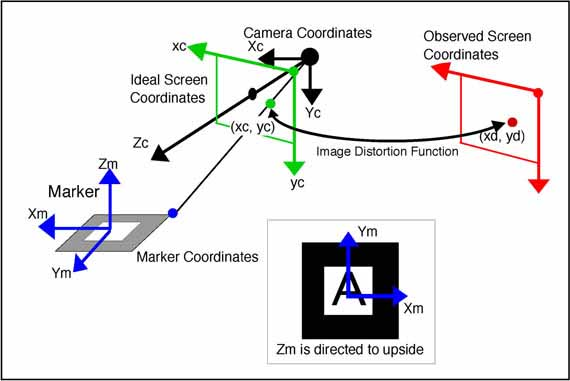
\includegraphics[width=0.7\linewidth]{Imagenes/ar-coordenadas}
	\caption{}
\label{ar-coordenadas}
\end{figure}


Otro detalle a considerar a la hora de calcular la matriz de la cámara, es la presencia de tres sistemas de coordenadas, el proyectado en la imagen de la cámara (2D), y los sistemas 3D de la cámara y el marcador.
	
\subsubsection{Estimacion matriz de la camara}
Los sistemas de coordenadas de la cámara y del marcador difieren entre si por la rotación y la trasalacion. La relación entre ambos puede ser descripta como:

\[
\begin{bmatrix}
X_{C} \\
Y_{C} \\
Z_{C} \\
1
\end{bmatrix} =
\begin{bmatrix}
R_{11} && R_{12} && R_{13} && T_{1} \\
R_{21} && R_{22} && R_{23} && T_{2} \\
R_{31} && R_{32} && R_{33} && T_{3} \\
0 && 0 && 0 && 1
\end{bmatrix}
\begin{bmatrix}
X_{M} \\
Y_{M} \\
Z_{M} \\
1
\end{bmatrix} = 
T_{CM} * \begin{bmatrix}
X_{M} \\
Y_{M} \\
Z_{M} \\
1
\end{bmatrix}
\]

Donde $ T_{CM} $ es la matriz de pose o la matriz de transformación de la cámara, la cual se utiliza para determinar la posición del objeto a aumentar con respecto en el sistemas de coordenadas de la cámara. Los valores de $T_{i}$ corresponden al vector de traslación, mientras que los nueve restantes $R_{ij}$ son parámetros obtenidos a partir de las 3 coordenadas de rotación.
Esta operación se realiza en cada frame donde un marcador es detectado.

Tal como se expresa en [4] luego del thresholding de la imagen, las regiones cuyos bordes exteriores pueden aproximarse mediante cuatro lineas son extraídas. A partir de estas cuatro lineas se extraen parámetros y las coordenadas de los cuatro vértices donde las mismas intersectan, los cuales se utilizan a futuro.

Estas regiones son normalizadas y su contenido interior es comparado utilizando \textit{template matching} con patrones para la identificación de la misma. Para este proceso de normalización se utiliza la matriz que se encuentra abajo, cuyas variables son determinadas por las coordenadas de los cuatro vértices detectados reemplazando las coordenadas en la imagen y en el sistema del marcador en $(x_{c},y_{c})$ y $(X_m,Y_m)$ respectivamente.

\[
\begin{bmatrix}
hx_{c} \\
hy_{c} \\
h 
\end{bmatrix} =
\begin{bmatrix}
N_{11} && N_{12} && N_{13}\\ 
N_{21} && N_{22} && N_{23}\\
N_{31} && N_{32} && 1
\end{bmatrix} 
\begin{bmatrix}
X_{m} \\
Y_{m} \\
1
\end{bmatrix}
\]

Como se expresa en [4] cuando dos lados paralelos de un marcados son proyectados en la imagen, las ecuaciones que representan a esas lineas en el sistema de coordenadas de la cámara son:
\begin{equation}
a_{1}x+b_1y + c_1 = 0
\end{equation}
\begin{equation}
a_{2}x+b_2y + c_2 = 0
\end{equation}
En donde los valores de estos parámetros son obtenidos durante el proceso de line-fitting. Dada la matriz de projeccion P que se obtiene durante la calibración de la cámara, las ecuación de los planos que incluyen estos dos lados del marcador, pueden ser representados en el sistema de coordenadas de la cámara reemplazando $x_c$ y $y_c$ por $x$ e $y$.

\begin{equation}
a_1P_{11}X_c + (a_1P_{12}+ b_1P_{22})Y_c + (a_1P_{13}+ b_1P_{23}+ c_1)Z_c = 0
\end{equation}
\begin{equation}
a_2P_{11}X_c + (a_2P_{12}+ b_2P_{22})Y_c + (a_2P_{13}+ b_2P_{23}+ c_2)Z_c = 0
\end{equation}

De esta manera obtenemos dos vectores normales, $ \textbf{n}_{1} $ y $ \textbf{n}_{2} $, a los planos que generan las lineas

\begin{figure}
	\centering
	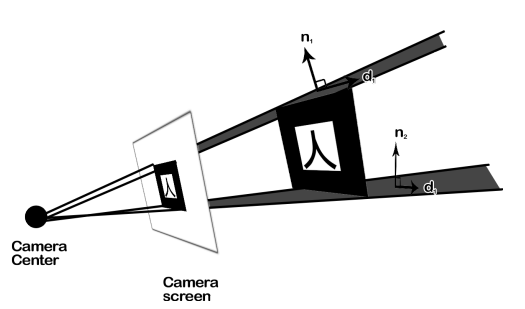
\includegraphics[width=0.7\linewidth]{Imagenes/ar-normales}
	\caption{}
	\label{fig:ar-normales}
\end{figure}

Como se expresa en [2] las variables $d_1$ y $ d_2 $ denotan los vectores de dirección de los lados del marcador, el cual al tener forma cuadrada, cada uno de los vectores representa la dirección de dos lados cada uno. Ya que $ d_1 $ esta proyectado sobre el plano de uno de los lados, esto significa que sera perpendicular a $ n_1 $ ya que $ n_1 X n_2 = d_1 $.

Sin embargo, tal como expresa [2] y [3], debido a errores en el procesamiento de la imagen, los vectores $d$ y $n$ no necesariamente seran exactamente perpendiculares. Para ellos se utilizan otros vectores $v_1$ y $ v_2 $, notese que el angulo entre $ v_1, d_1 $ es igual al de $v_2,d_2$. A partir de $v_1$ y $ v_2 $ obtenemos $ v_3 $ realizan el producto cartesiano para obtener un vector perpendicular $v_3$. Estos tres vectores componen el componente de rotacion de la matriz de transofrmacion $\textbf{T}_CM$

\begin{figure}
	\centering
	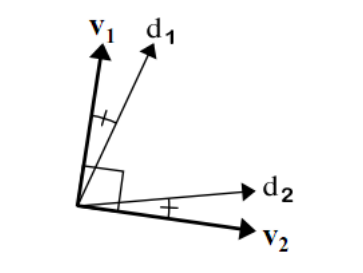
\includegraphics[width=0.7\linewidth]{Imagenes/ar-d1d2}
	\caption{}
	\label{fig:ar-d1d2}
\end{figure}

Para la obtención de los parametros de traslación, basta con resolver el sistema de ecuaciones que se definen en la relación entre las coordenadas de los cuatro vertices en el sistema de coordenadas de la imagen de la camara y el sistema de coordenadas del marcador.

como expresa [4] este metodo de obtencion de la matriz de transformacion puede incluir errores, los cuales pueden reducirse utilizando la matriz ya obtenida para poder transformar las coordenadas de los vertices del marcador que estan en el sistema de coordenadas del mismo, al sistema de coordenadas de la imagen de la camera. Luego esta matriz de transformacion es optimizada  con la suma de las diferencias entre las coordenadas transformadas y las coordenadas obtenidas desde la imagen. De esta forma se optimizan los componentes de rotacion de la mtriz (ya que solo hay seis varibales independientes), para reestimar los componentes de traslacion se utiliza el metodo descripto anteriormente. 



La relación entre las coordenadas de la imagen de la camara y y las coordenadas de la camara esta definida por:
\[
\begin{bmatrix}
hX_{1} \\
hY_{1} \\
h 
\end{bmatrix} =
\begin{bmatrix}
P_{11} && P_{12} && P_{13} && 0\\ 
0 && P_{22} && P_{23} && 0\\
0 && 0 && 1 && 0
\end{bmatrix} 
\begin{bmatrix}
X_{C} \\
Y_{C} \\
Z_{C} \\
1
\end{bmatrix} = P \begin{bmatrix}
X_{C} \\
Y_{C} \\
Z_{C} \\
1
\end{bmatrix}
\]

donde $P$ se denomina \textit{intrinsic camera parameters}, la cual es camara dependiente. En el caso de ARToolKit esta misma esta definida como:

\[
\begin{bmatrix}
s_{x}f && 0 && x_{0} && 0\\ 
0 && s_{y}f && y_{0} && 0\\
0 && 0 && 1 && 0
\end{bmatrix} 
\]

donde $f$ es la longitud focal de la camara, $s_{x}$ el factor de escala en el eje $x$, $s_{y}$ el factor de escala en el eje $y$ y por último $(x_{0},y_{0})$ es la posicion donde el eje $z$ del sistema de coordenadas de la camara \textit{frame passes}
	
	
	\subsection{Pose calculation}
	
	Dada las caracteristicas de las camaras modernas,podemos asumir que la distorsion puede ser separada del modelo de la camara. Aquellos puntos que pertenecen a las coordenadas sin distorsion %$\textbf{x_{i}}$ y los pertenencientes a las coordenadas del sistema del marcado como $\textbf{X_{i}}$.
	%El proceso de deteccion de marcadores nos brinda las coordenadas de las esquinas del mismo  $\textbf{x_{1},x_{2},x_{3},x_{4}}$

\subsection{asd}
las coordenadas reales de las esquinas son conocidas. El sistema poee ocho ecuaciones, una para cada una de las coordenadas que componen los cuatro puntos de las esquinas, y 6 parametros libres. Esto posibilita la estimacion de la matriz de transformación.

Un approach comunmente usado es utiliza metodos no iterativos para obtener una estimacion inicial de la pose, por ejemplio DTL direct linear transformation, y luego utilizar una optimizacion iterativa para calcular la pose exacta.

Se reproyecta el mundo X en el plano de la imagen, utilizando la matriz estimada $M^{'}$, definimos el punto reproyectado $x^{'}$
\begin{equation}
x^{'}= M^{'}X
\end{equation}

Se puede resolver la matriz de tranformacion encontrando una matriz que miniza el error de proyecccion $||x - x^{'}||$ 

\begin{equation}
err = \frac{1}{4} \sum {i=1}{4}
\end{equation}

Este es un problema de estimacion no-lineal y el sistema puede resolverse analogamente a la calibracion de la camera utilizando el metodo iterativo Levenberg

La optimizacion de lerror de reproyeccion es un metodo rapido y es utilizado por ARToolKit. En el modo de trackeo continuo, ARToolKit combina esta tecnicae con los resultados de tracking del frame anterior [83]

\subsubsection{Template matvhing}
Template markers son marcados en blanco y negro que contienen una imagen simple dentro de bordes negros. El sistema de deteccion identifica los marcados comparandolos con markers template, son ejemplos de marcadores, los cuales tienen un nombre o id unico que los identifica. De esta manera se elija la mayor comparacion.

La identificacion de marcadores es una version simplificada del problema de template matching, ya que en la deteccion de marcadore el area de matching eta definida, mientras que en el problema general, la ubicacion, tamaño y orientacion de la matching area no son conocdas.

En template matching, el marcador detectado es unwarped utilizando la pose de la camara calculada, escalando al tamaño del template el marcador y comparando en cuatro posicione diferentes el marcador con los distintos templates. El template que da el mayor valor de similitud (el menor de disimilitud) e el marcador correcto, adicionalmente obteniendo la orientacion correcta.

Si todos los valores de similitud son menores al trheshold el sistema descarta el marcador.

En lugar de unrwrapping todo el marcador, el sistema puede proyectar los centros de las cells en el template a las coordenadas de la magen utilizando la pose de la camara calculada. Luego los valores de los pixeles se puede obtener directamente de la imagen en escala de gris o threshold. El valor de los pixeles se puede coniderar como el valor del pixel mas cercano, el promerio de los N vecinos.


Antes del template matching, generalmente, una imagen en escala de gris es normalizada de modo que aquellas zonas oscuras quedan en negro y las claras en blanco.

el valor de similitud puede basarse en SSD (suma de diferencias de cuadrados) or cross-correlation


\bibliography{biblio}{}
\bibliographystyle{plain}

\end{document}
